\documentclass[extendedabs]{bmvc2k}
\usepackage[ruled]{algorithm2e}
\usepackage{amsmath}
\begin{document}

\title{Digital Image Processing HW4}
\addauthor{Hejung Yang}{}{1}
\addinstitution{School of Electrical and Electronic Engineering, 
Yonsei University.}

\maketitle
\vspace{-0.2in}

\section*{problem 1: edge detection}

\begin{figure}[h]
    \centering
    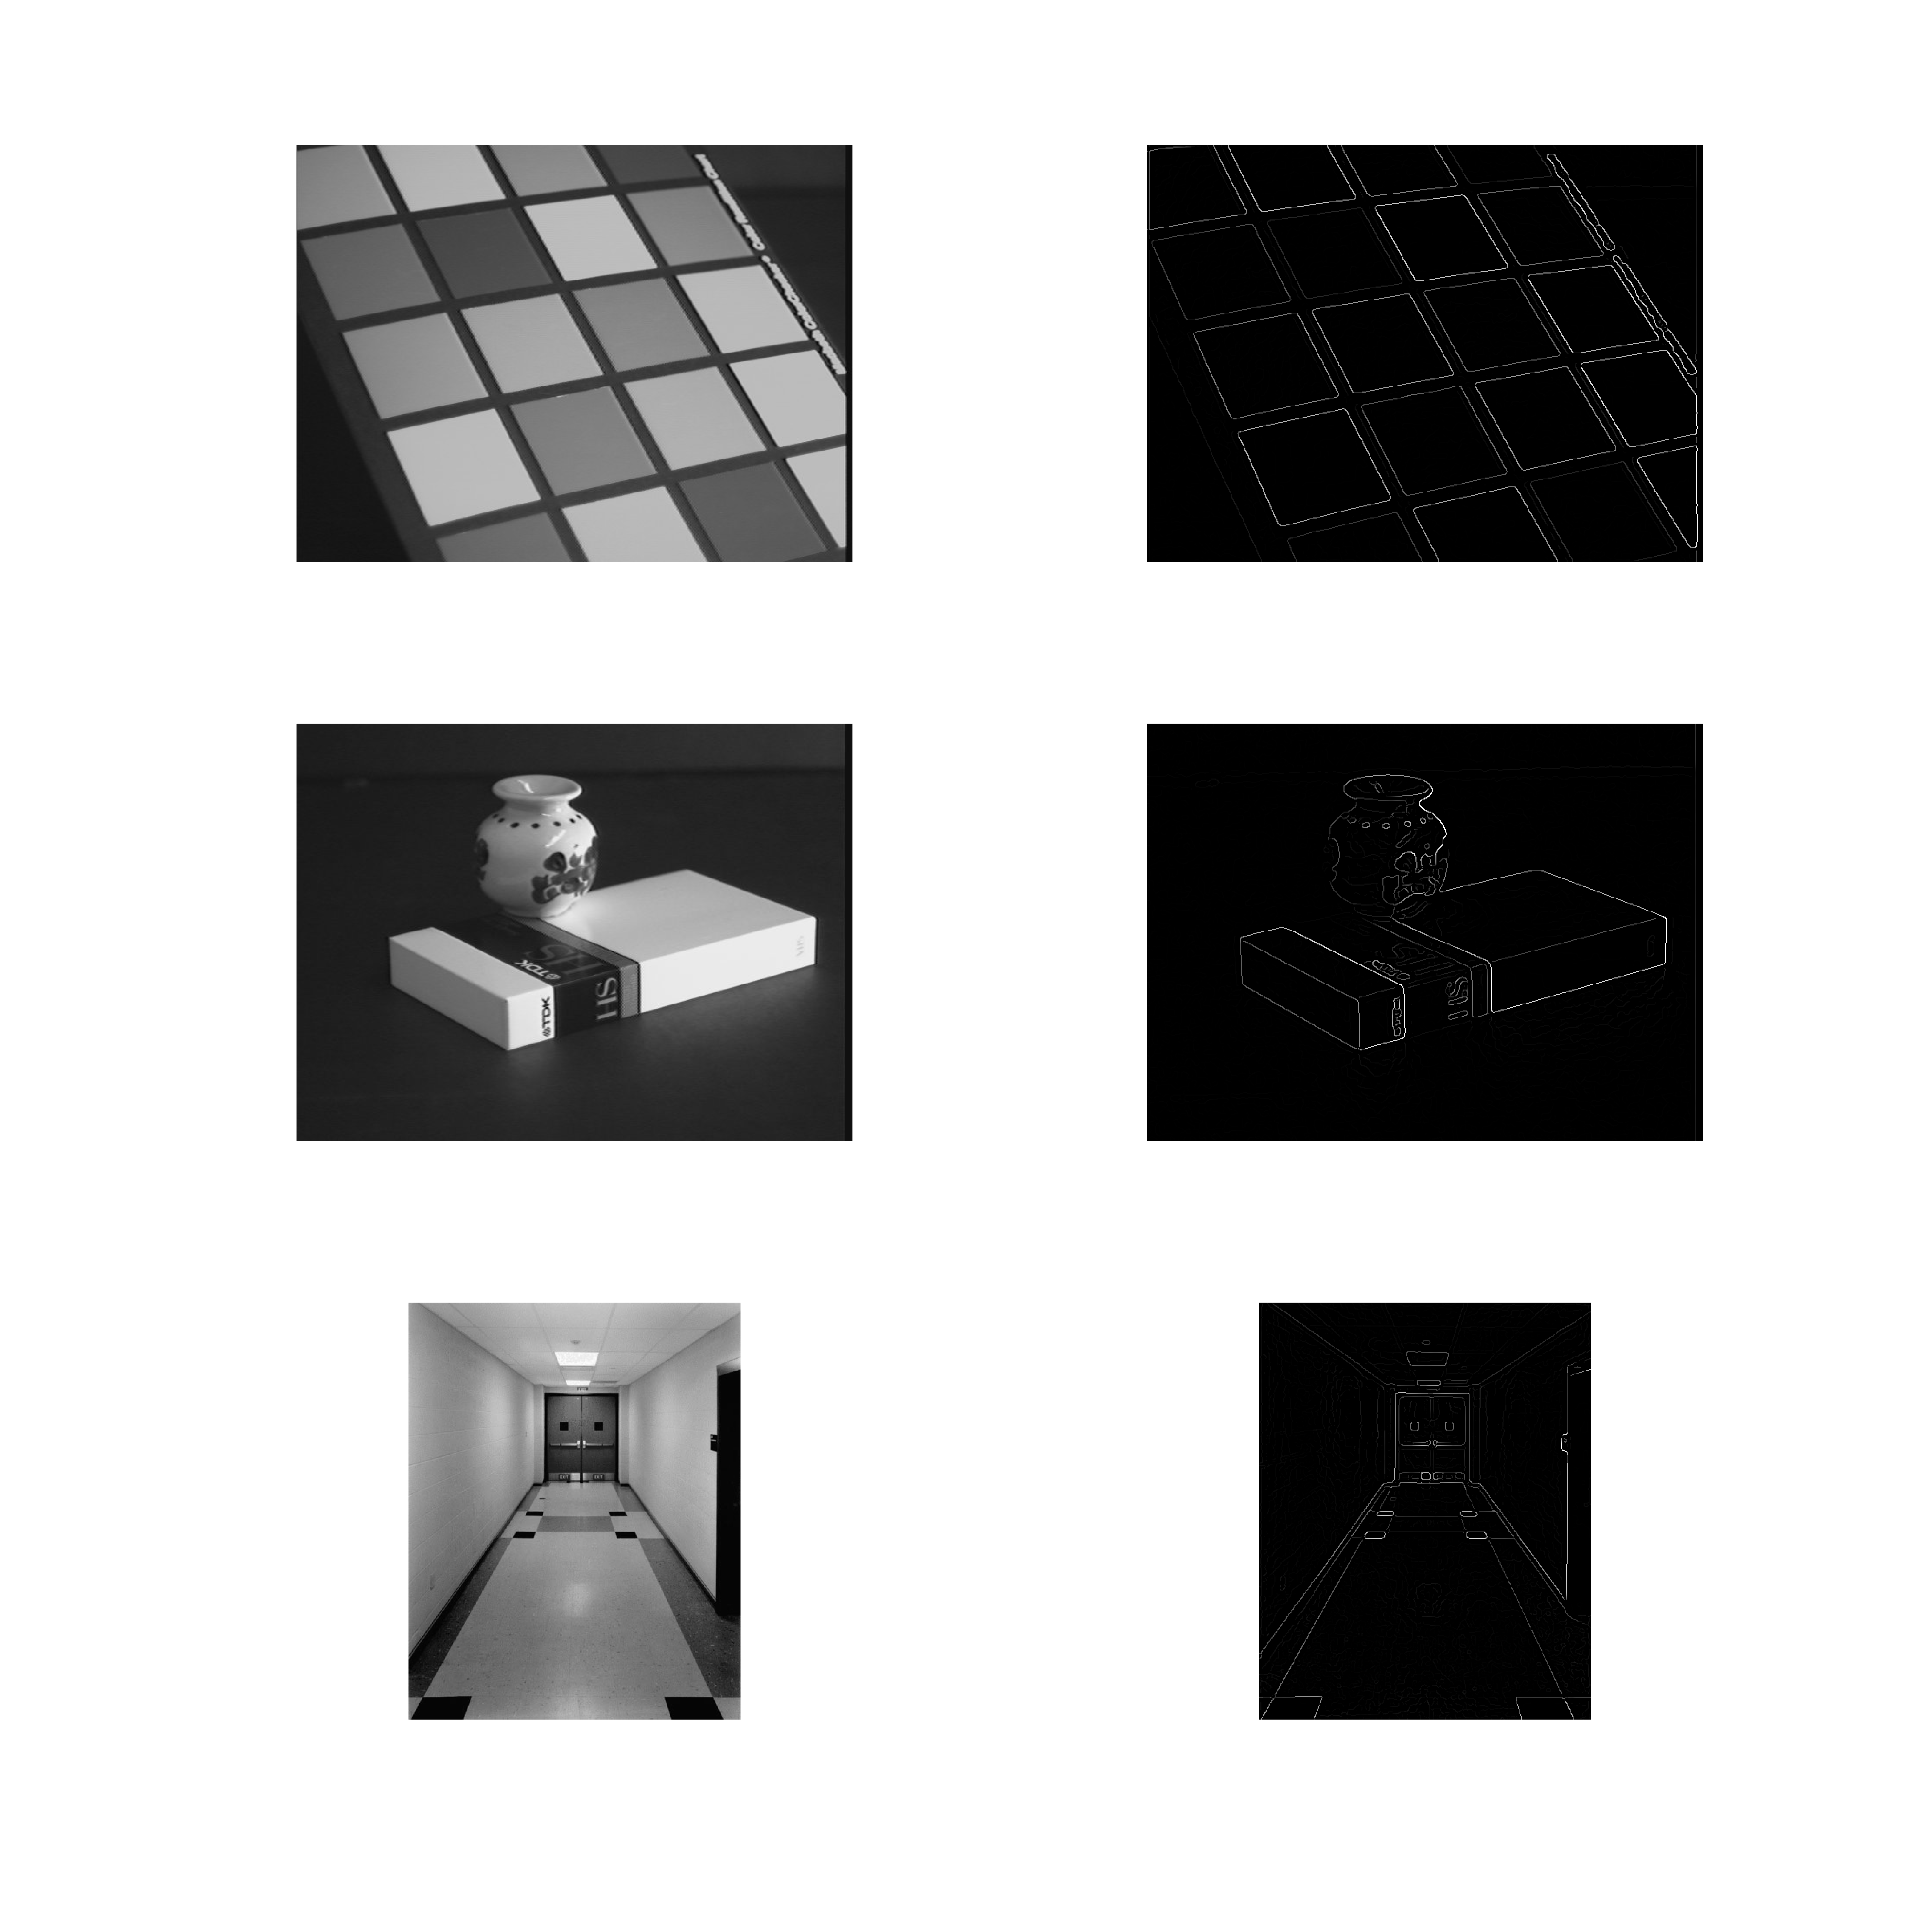
\includegraphics[width=\linewidth]{hw4_1_1}
    \caption{result of edge detection(right) given image(left)}
    \label{fig:1}
\end{figure}

Matlab code matlab/myEdgeFilter.m contains edge detection routine given greyscale image and standard deviation
of the gaussian kernel for smoothing the image before edge detection. Edge detection is composed of three stages;
first, the image is smoothed out so to prevent the noise to be detected as an edge component. Smoothing is done with
gaussian filter with the specified standard deviation. Next, Sobel filter is applied onto the smoothed image. In detail,
two first derivative filters, known as Sobel mask $S_x$, $S_y$ for horizontal/vertical changes, are applied onto the image. 

\[S_x = \begin{bmatrix}-1 & -2 & -1\\ 0 & 0 & 0\\ 1 & 2 & 1\end{bmatrix} , \quad
S_y = \begin{bmatrix}-1 & 0 & 1\\ -2 & 0 & 2\\ -1 & 0 & 1\end{bmatrix}\]
\[G_x = S_x \ast image , \quad G_y = S_y \ast image\]

The output are horizontal and vertical derivative approximations of the image, $G_x$ and $G_y$ respectively. 
Magnitude, angle gradient of the image $M$, $\alpha$ can be calculated with the equation below:

\[M = \sqrt{G_x^2 + G_y^2}\]
\[\alpha = tan^{-1}(\frac{G_y}{G_x})\]

Lastly, with non-maximum suppression (NMS), weak magnitude within a window is suppressed, producing thinner edge components.
NMS is processed as follows: for each pixel position $(x,y)$, its magnitude gradient $M(x,y)$ is compared with the magnitude of
its neighboring pixels in direction $\alpha(x,y)$ within a window. If $M(x,y)$ is smaller than any of the magnitudes along the
gradient line, $M(x,y)$ is suppressed.

Algorithm\ref{alg:1} shows the pseudo code for the NMS logic. For the implementation, angle gradient $\alpha$ is rounded to
one of 8-directions, east, north-east, north, north-west, west, south-west, south, south-east and then based on the direction,
the magnitudes of the pixels along the direction are compared with the center magnitude value to decide whether to suppress the
center magnitude gradient or not.

\begin{algorithm}
    \caption{non-maximum suppression}
    \label{alg:1}
    \KwIn{$M$ of size $(M,N)$}
    \KwIn{$\alpha$ of size $(M,N)$}
    $processed_M = M$\;
    \For{$i = 1:M$}{
        \For{$j = 1:N$}{
            round angle $\alpha(i,j)$ by one of the direction:
            {east, north-east, north, north-west, west, south-west, south, south-east}\;
            \If{rounded angle is east or west}{
                \If{$M(i,j) < M(i,j+1)$ or $M(i,j) < M(i,j-1)$}{
                    $processed_M(i,j) = 0$\;
                }
            }
            \If{rounded angle is north-east or south-west}{
                \If{$M(i,j) < M(i+1,j-1)$ or $M(i,j) < M(i-1,j+1)$}{
                    $processed_M(i,j) = 0$\;
                }
            }
            \If{rounded angle is north or south}{
                \If{$M(i,j) < M(i+1,j)$ or $M(i,j) < M(i-1)$}{
                    $processed_M(i,j) = 0$\;
                }
            }
            \If{rounded angle is north-west or south-east}{
                \If{$M(i,j) < M(i+1,j+1)$ or $M(i,j) < M(i-1,j-1)$}{
                    $processed_M(i,j) = 0$\;
                }
            }
        }
    }
    return $processed_M$\;
\end{algorithm}

\begin{figure}[h]
    \centering
    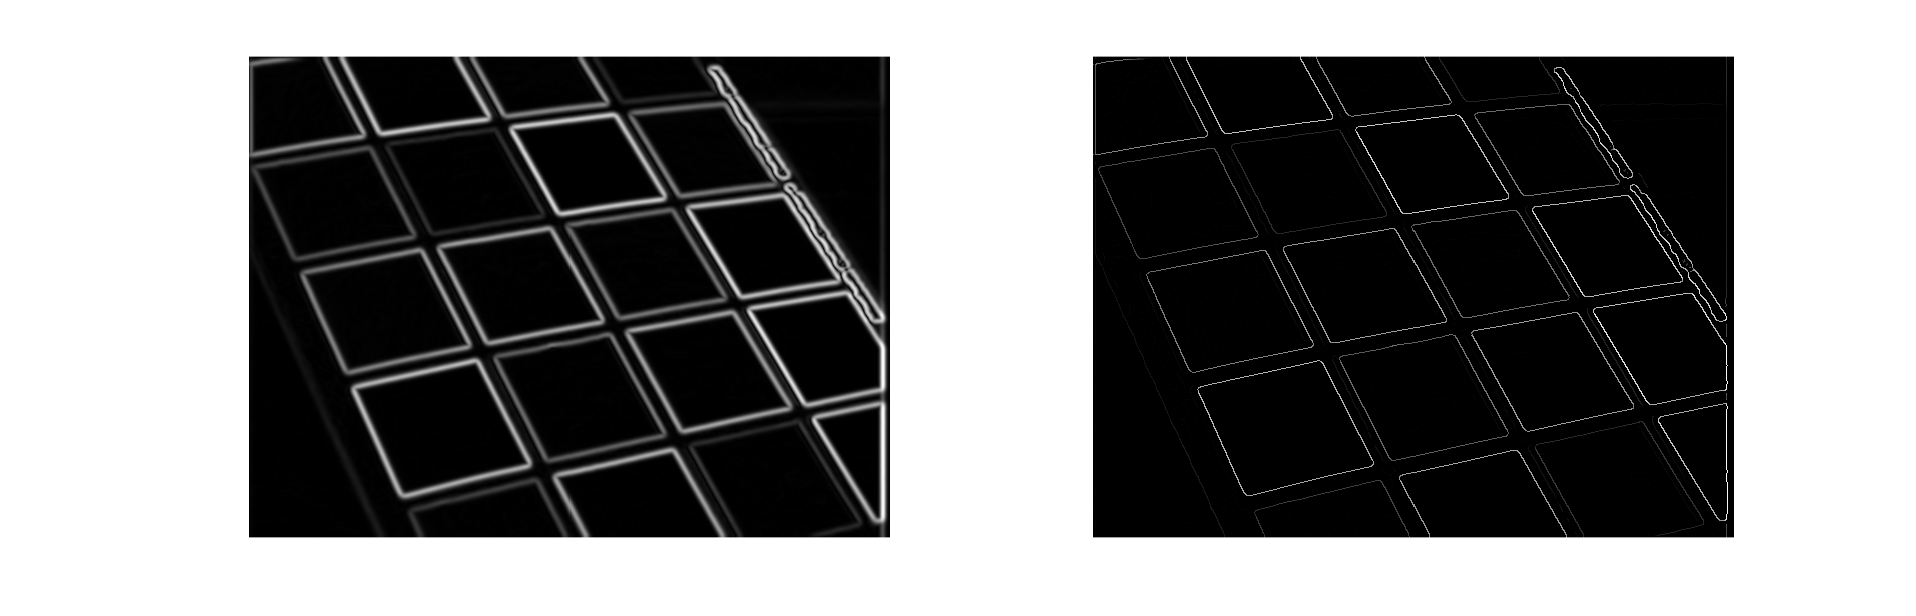
\includegraphics[width=\linewidth]{hw4_1_2}
    \caption{result of edge detection without NMS(left) and with NMS(right)}
    \label{fig:2}
\end{figure}

\figurename{\ref{fig:2}} contains the edge detection results of the given image with or without the NMS postprocessing.
It can be seen that compared to the original(left), postprocessed image(right) has much thinner edge components.

\begin{figure}[h]
    \centering
    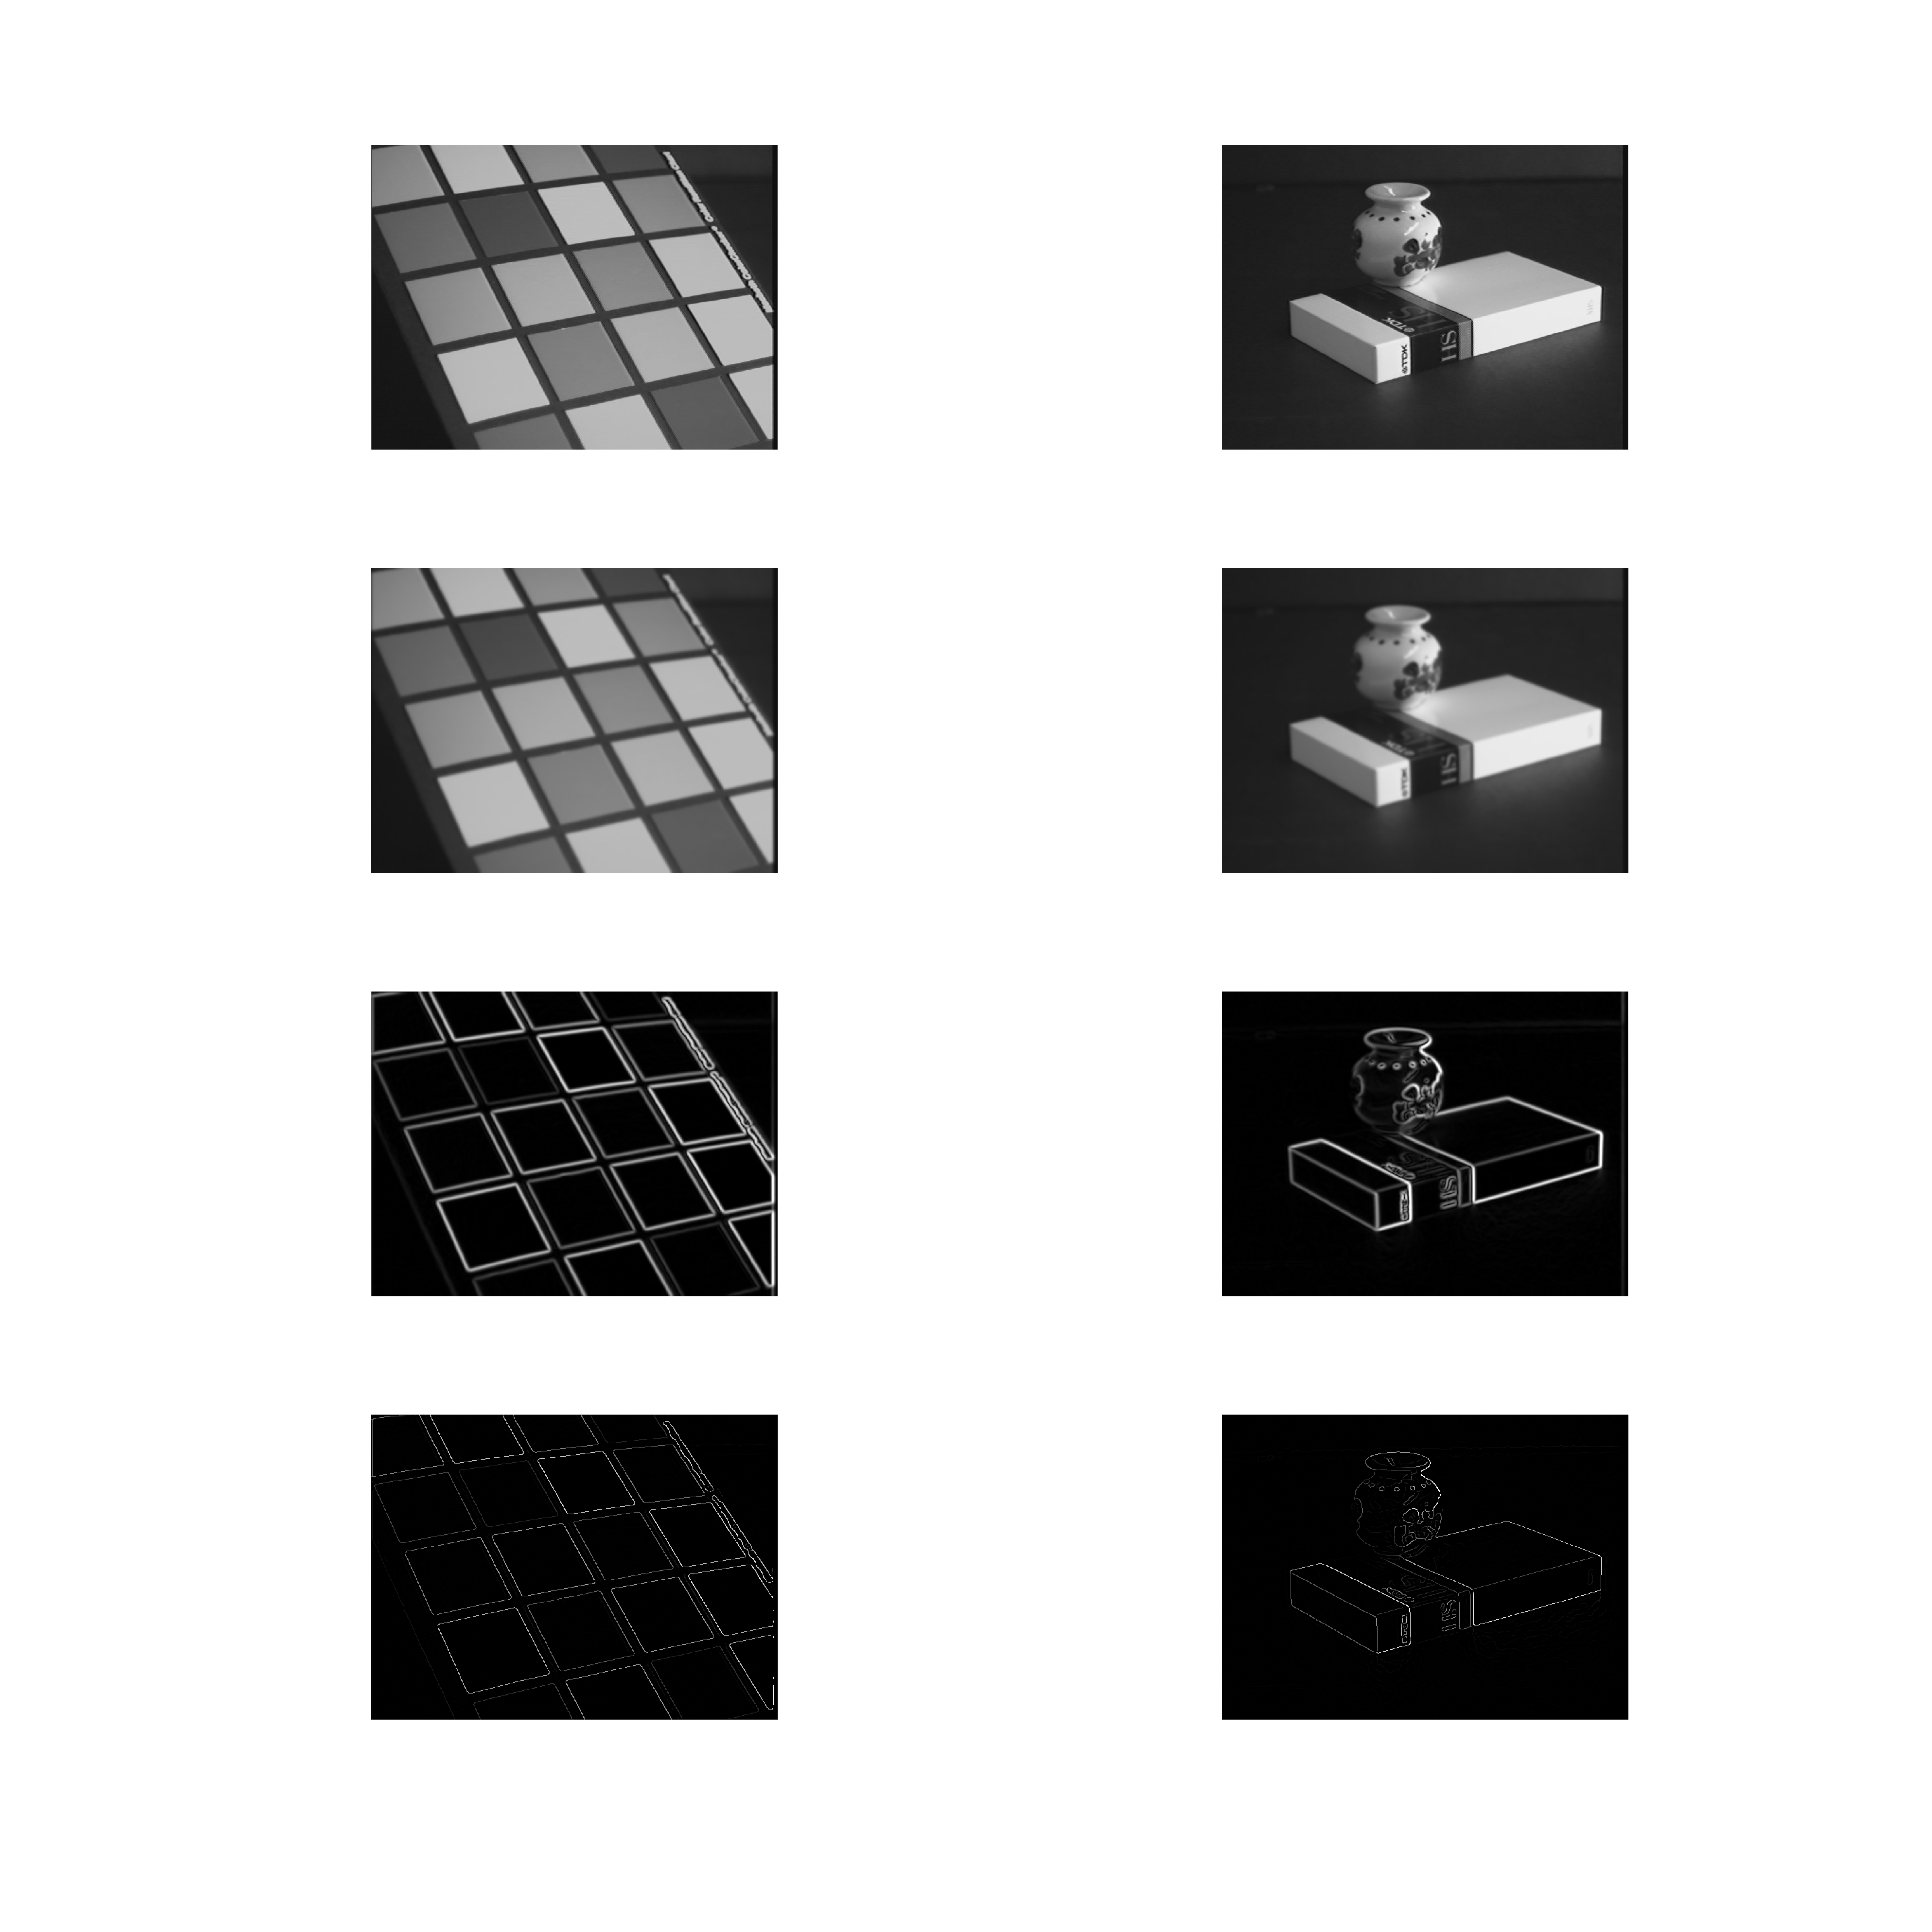
\includegraphics[width=\linewidth]{hw4_1_3}
    \caption{partial results of edge filtering step by step; first row: original image, second row:
    result of applying gaussian filter onto the image, third row: magnitude gradient of the smoothed image,
    fourth row: after applying NMS onto the magnitude image}
    \label{fig:10}
\end{figure}

\figurename{\ref{fig:10}} shows the partial results of applying matlab/myEdgeFilter.m step by step.
Applying gaussian filter generates smoothed image, followed by convolving Sobel masks and calculating magnitude of
the gradients. By NMS along the gradient line, the thick edge components become thinner.

Output edge component results given several images can be found in \figurename{\ref{fig:1}}.
It can be seen that various types of edges, ranging from straight lines to curves, isolated components like circles,
are successfully extracted. Remaining results of the edge detection from the images in data/ can be found in
results/*\_01edge.png. 

\section*{problem 2: the hough transform}

Matlab code matlab/myHoughTransform.m contains hough transform routine given edge image, threshold for ignoring small edge
filter response, resolution units for $\rho$ and $\theta$ for quantization. The implementation is based on the
Standard Hough Transform(SHT) that uses the parametric representation of a line as follows:
\[\rho = x * cos(\theta) + y*sin(\theta)\]

here $\rho$ is the distance between the line and the origin, $\theta$ is the angle of the projection from the origin to the line. 
\figurename{\ref{fig:3}} depicts the parametrization of a line in both planes. It can be seen that every line candidates that 
passes through each point in xy-plane can be represented as a sinusoidal curve in $\rho\theta$-plane.  

\begin{figure}[h]
    \centering
    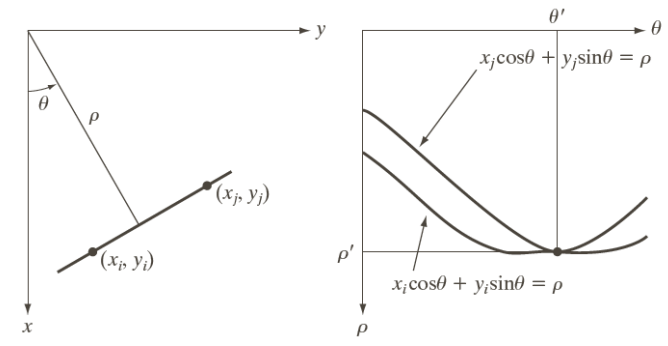
\includegraphics[width=\linewidth]{hw4_2_1}
    \caption{visualization of the parametric representation of a line in both xy-plane or $\rho\theta$-plane}
    \label{fig:3}
\end{figure}

As can be seen in \figurename{\ref{fig:3}}, intersection of the sinusoidal curves in $\rho\theta$-plane represents the common
line that passes through the points in $xy$-plane; The main goal for hough transformation is to find the maximum intersection 
occurs among the various sinusoidal curves mapped from points in $xy$-plane so that the line that penetrates most of the points
in $xy$-plane can be found. 

However it can be too exhaustive to find every intersections because $\rho$ and $\theta$ are both continuous values;
thus practical hough transform implementation given thresholded edge filter response starts with 
building valid $\rho$ and $\theta$ values with the resolution parameters. 

Followed by the MATLAB 
implementation, in matlab/houghTransform.m, max/min values for the $\rho$ are defined as:
\[D = \sqrt{(h-1)^2 + (w-1)^2}\]
\[min_{\rho} = -res_{\rho} * ceil(D / res_{\rho})\]
\[max_{\rho} = res_{\rho} * ceil(D / res_{\rho}) \]
where $h$, $w$ is the height, width of the given image and $res_{\rho}$ is the resolution unit of the $\rho$.
Thus, the valid values for $\rho$ and $\theta$, referred as $scale_{\rho}$ and $scale_{\theta}$ are 
defined as below. Notice that $\theta$ is degree value in below equation.
\[scale_{\rho} = min_{\rho}:res_{\rho}:max_{\rho}\]
\[scale_{\theta} = -90^\circ:res_{\theta}:90^\circ-res_{\theta}\]

$scale_{\theta}$ ranges from $-90^\circ$ to $90^\circ$ so that the line angle can cover every direction; if the 
parametric representation is of linear equation as:
\[y = ax + b\]
then it would have been impossible to parameterize vertical line, having infinite slope in linear equation.

With the valid list of $\rho$ and $\theta$ defined as $scale_{\rho}$ and $scale_{\theta}$, 
to find the intersections in $\rho\theta$-plane, mapping a continuous
sinusoidal curve of $\rho\theta$-plane into quantized points in $sclae_{\rho}$, $scale_{\theta}$ and 
accumulate each points so to find the maximum intersection is needed.

Accumulation of intersections on quantized $\rho\theta$-plane works as follows: the hough transform matrix $H$ is defined as 
$length(scale_{\theta}) \times length(scale_{\rho})$, initially set to zero.
Then, for every pixel position $(x,y)$ in the given edge response image, $\rho = x * cos(\theta) + y * sin(\theta)$ is calculated
for every $\theta$ in $scale_{\theta}$. $\rho$ is approximated as the value in $scale_{\rho}$, and $H(i_{\theta}, i_{\rho})$ is 
increased by 1 where $scale_{\theta}(i_{\theta}) = \theta$, $scale_{\rho}(i_{\rho}) = \rho$. 

Resulting matrix $H$ contains the hough transform accumulator containing the number of intersections found in quantized 
$\rho\theta$-plane, in other words, the number of votes for having a line with the given parameter $\rho$, $\theta$ in 
$xy$-plane thoughout the edge response image.

\begin{algorithm}
    \caption{acuumulation on parametric representation}
    \label{alg:3}
    \KwIn{$Image$ of size $(M,N)$}
    \KwIn{$scale_{\rho}$}
    \KwIn{$scale_{\theta}$}
    $H = zeros(length(scale_{\theta}), length(scale_{\rho})))$\;
    \For{$i = 1:M$}{
        \For{$j = 1:N$}{
            \If{$Image(i,j)$}{
                \For{$theta\_idx = 1:length(scale_{\theta})$}{
                    $theta = scale_{\theta}(theta\_idx)$\;
                    $rho = (n-1) * cos(theta) + (m-1) * sin(theta)$\;
                    convert $rho$ into scale index $rho\_idx$\;
                    $H(theta\_idx, rho\_idx) = H(theta\_idx, rho\_idx) + 1$\;
                }
            }
        }
    }
    return $H$\;
\end{algorithm}
Algorithm\ref{alg:3} contains the pseudo-code routine for accumulating intersections as described above.

\begin{figure}[h]
    \centering
    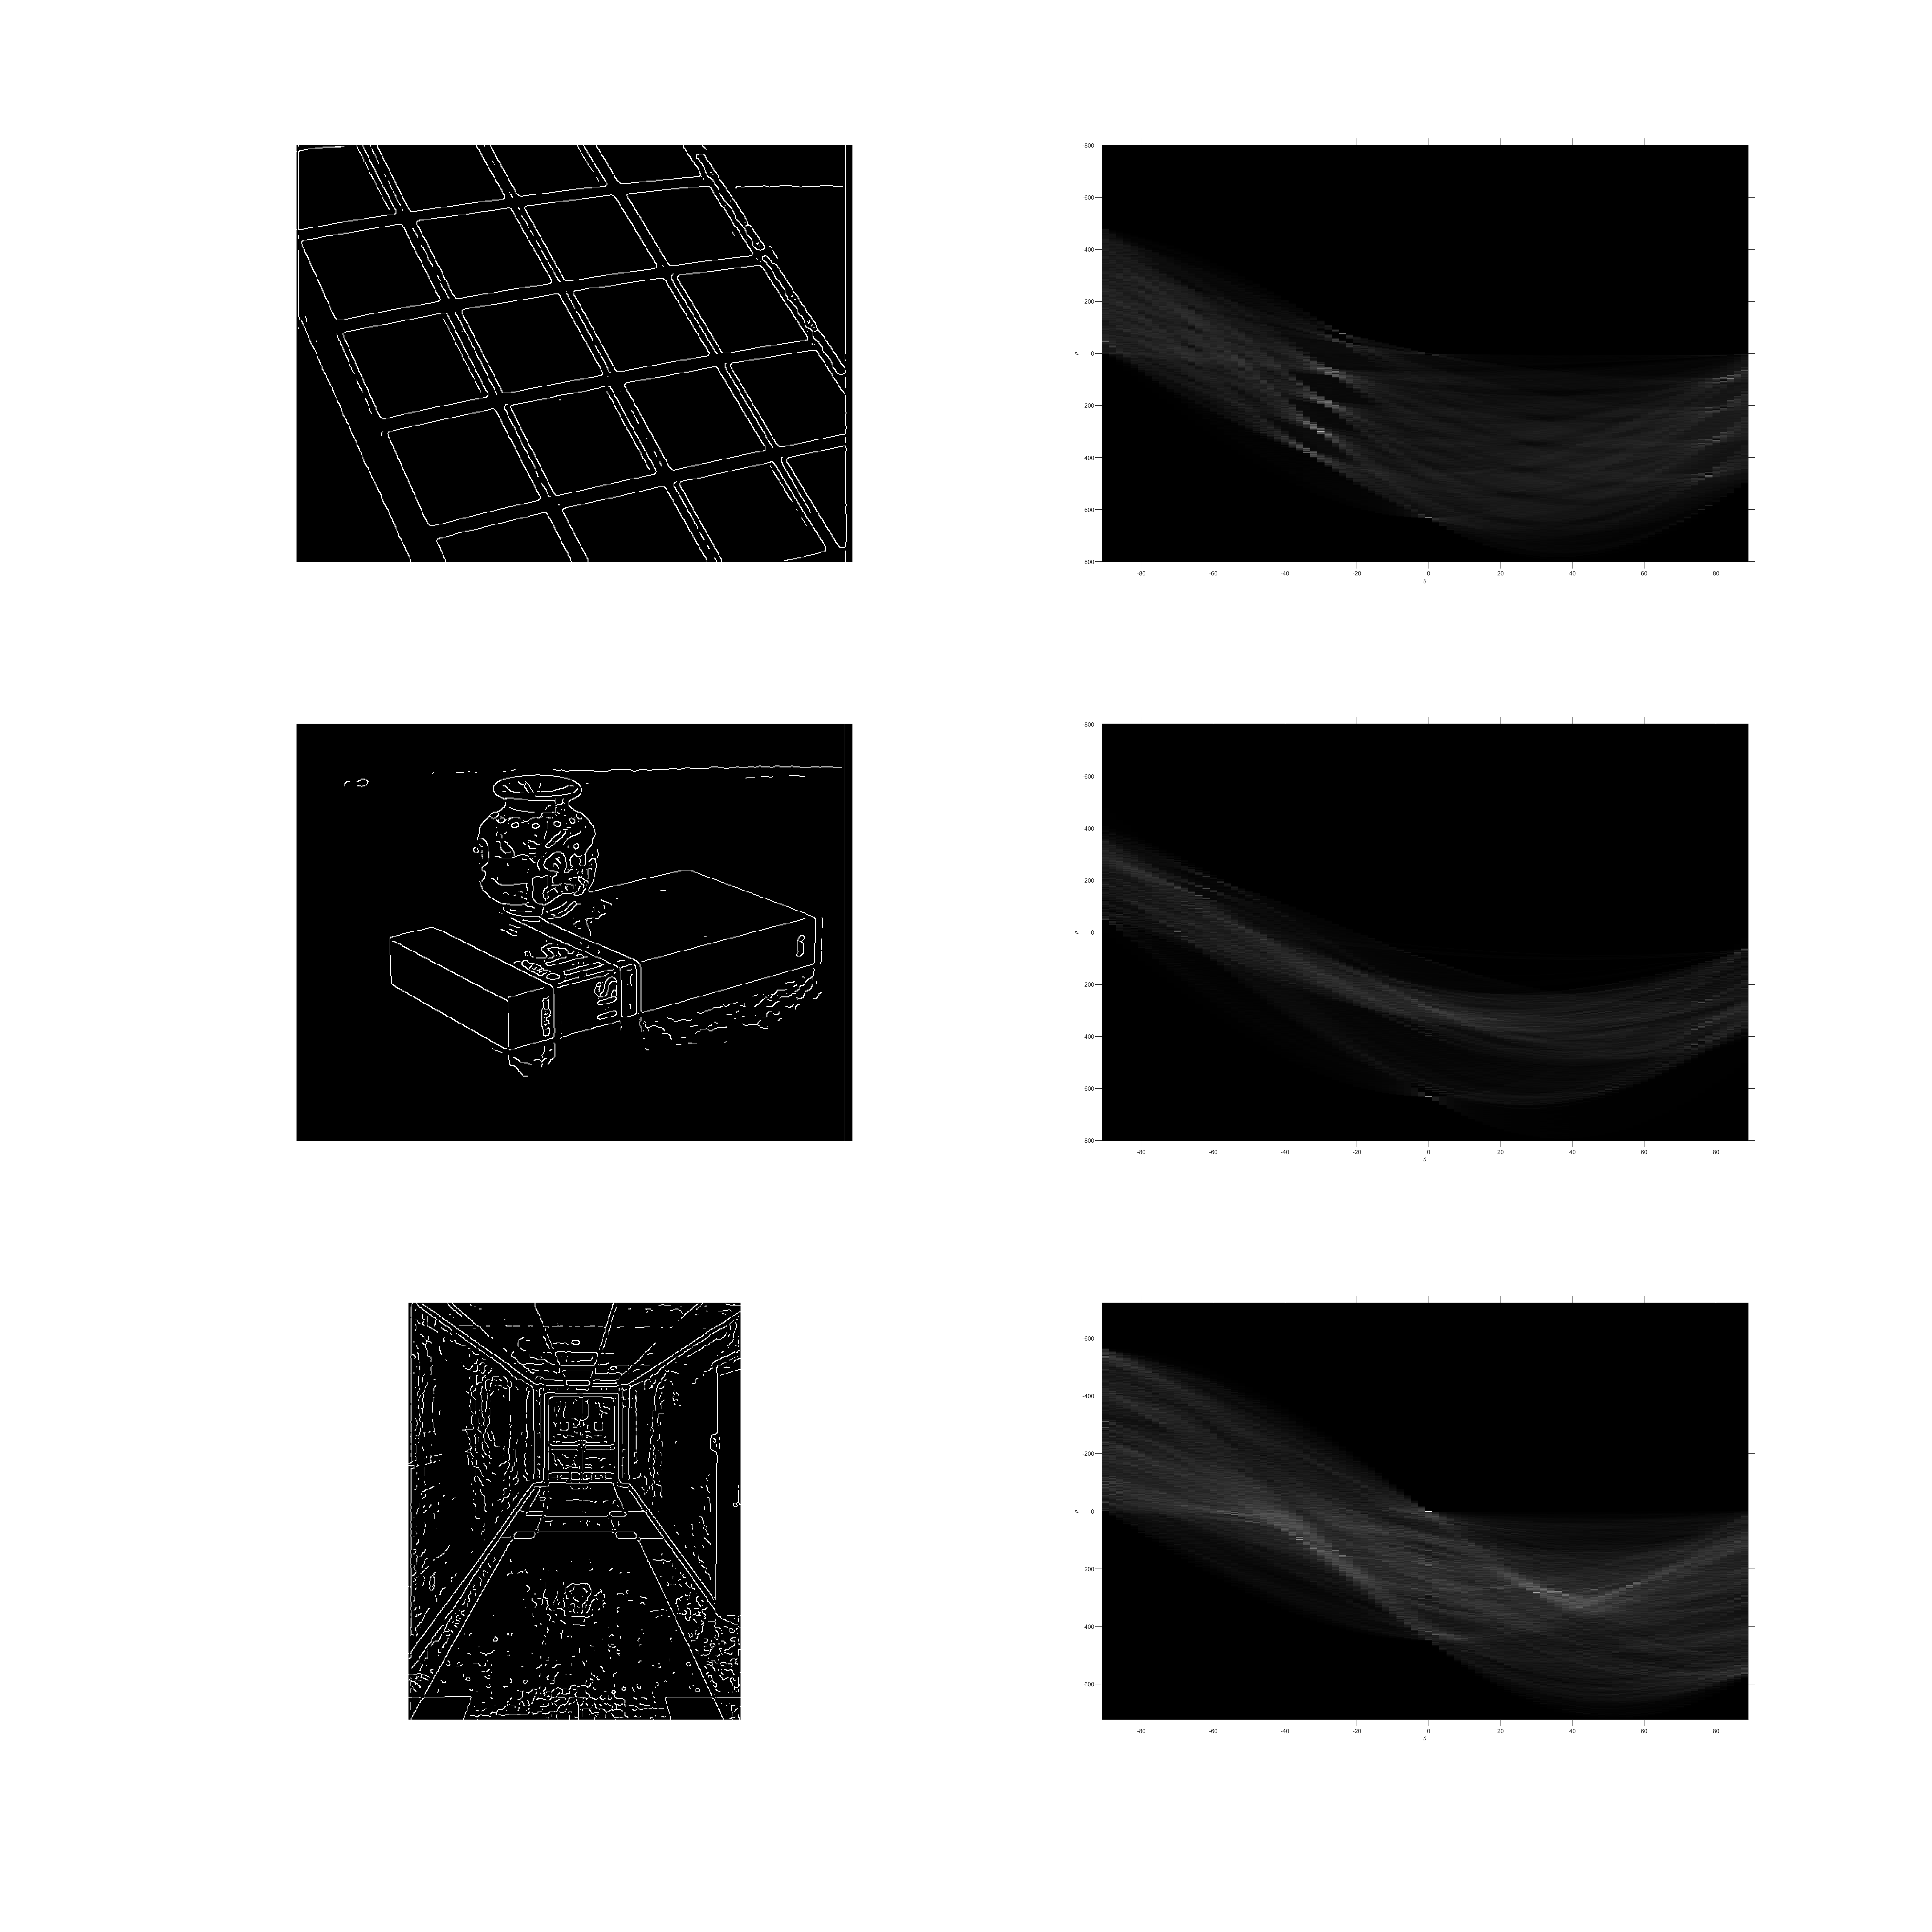
\includegraphics[width=\linewidth]{hw4_2_2}
    \caption{edge response and its hough transform of the given image. $res_{\rho} = 2$, $res_{\theta} = 2^{\circ}$
    is used for hough transformation}
    \label{fig:4}
\end{figure}

\figurename{\ref{fig:4}} depicts the hough transform given edge response images. Depending on the image, the range
containing high accumulator value differs. In first row of \figurename{\ref{fig:4}}, at $\theta$ range from $-40^\circ$ to $-20^\circ$, high accumulation
is observed which can be one of the major lines. On the other hand, at third row, high accumulations are largely observed
in $\theta$ range from $-40^\circ$ to $60^\circ$. This can indicate two things; there can be many noisy edge responses, or
it can produce some thick lines. To reduce unwanted noisy lines, postprocessing can be done in next section.

Remaining results of the hough transformation from the images in data/ can be found in
results/*\_03hough.png. 

\section*{problem 3: finding lines}

Matlab code matlab/myHoughLines.m accepts the hough transform matrix $H$ and the number of peaks to be extracted as input
arguments and returns the peak coordinates within $H$. The peak in $\rho\theta$ plane corresponds to a line in $xy$ plane.

Naive implementation of returning $\rho\theta$ indices of top $N$ values in $H$ where $N$ refers to the maximum number of
peaks to be found can generate thick lines, unwanted noises. Non-maximum suppression on $\rho\theta$ plane can help with
thinner lines while suppressing noisy lines. NMS can be done as follows: For each iteration, select the index 
$(i_{\rho} i_{\theta})$ from $H$ having the maximum value, and then set $H(i, j)$ as $0$ where $(i, j)$ is the indices 
within the window centered at $(i_{\rho}, i_{\theta})$.

Detailed algorithm can be found in Algorithm\ref{alg:2}.

\begin{algorithm}
    \caption{matlab/myHoughLines.m}
    \label{alg:2}
    \KwIn{$H$ of size $(M,N)$}
    \KwIn{$numLines$}
    $peaks = zeros(nLines, 2)$\;
    $threshold = 0.3 * max(H(:))$\;
    $radius = [4, 4]$\;
    \For{$i = 1:nLines$}{
        $[val, idx] = max(H(:))$\;
        \If{$val < thres$}{
            break\;
        }
        $[i_{\rho}, i_{\theta}] = ind2sub(size(H), idx)$\;
        push $[i_{\rho}, i_{\theta}]$ in $peaks$\;
        \For{$j = i_{\rho} - radius(1) : i_{\rho} + radius(1)$}{
            \For{$k = i_{\theta} - radius(2) : i_{\theta} + radius(2)$}{
                $H(j, k) = 0$\;
            }
        }
    }
    return $peaks(:, 1), peaks(:, 2)$\;
\end{algorithm}

\begin{figure}[h]
    \centering
    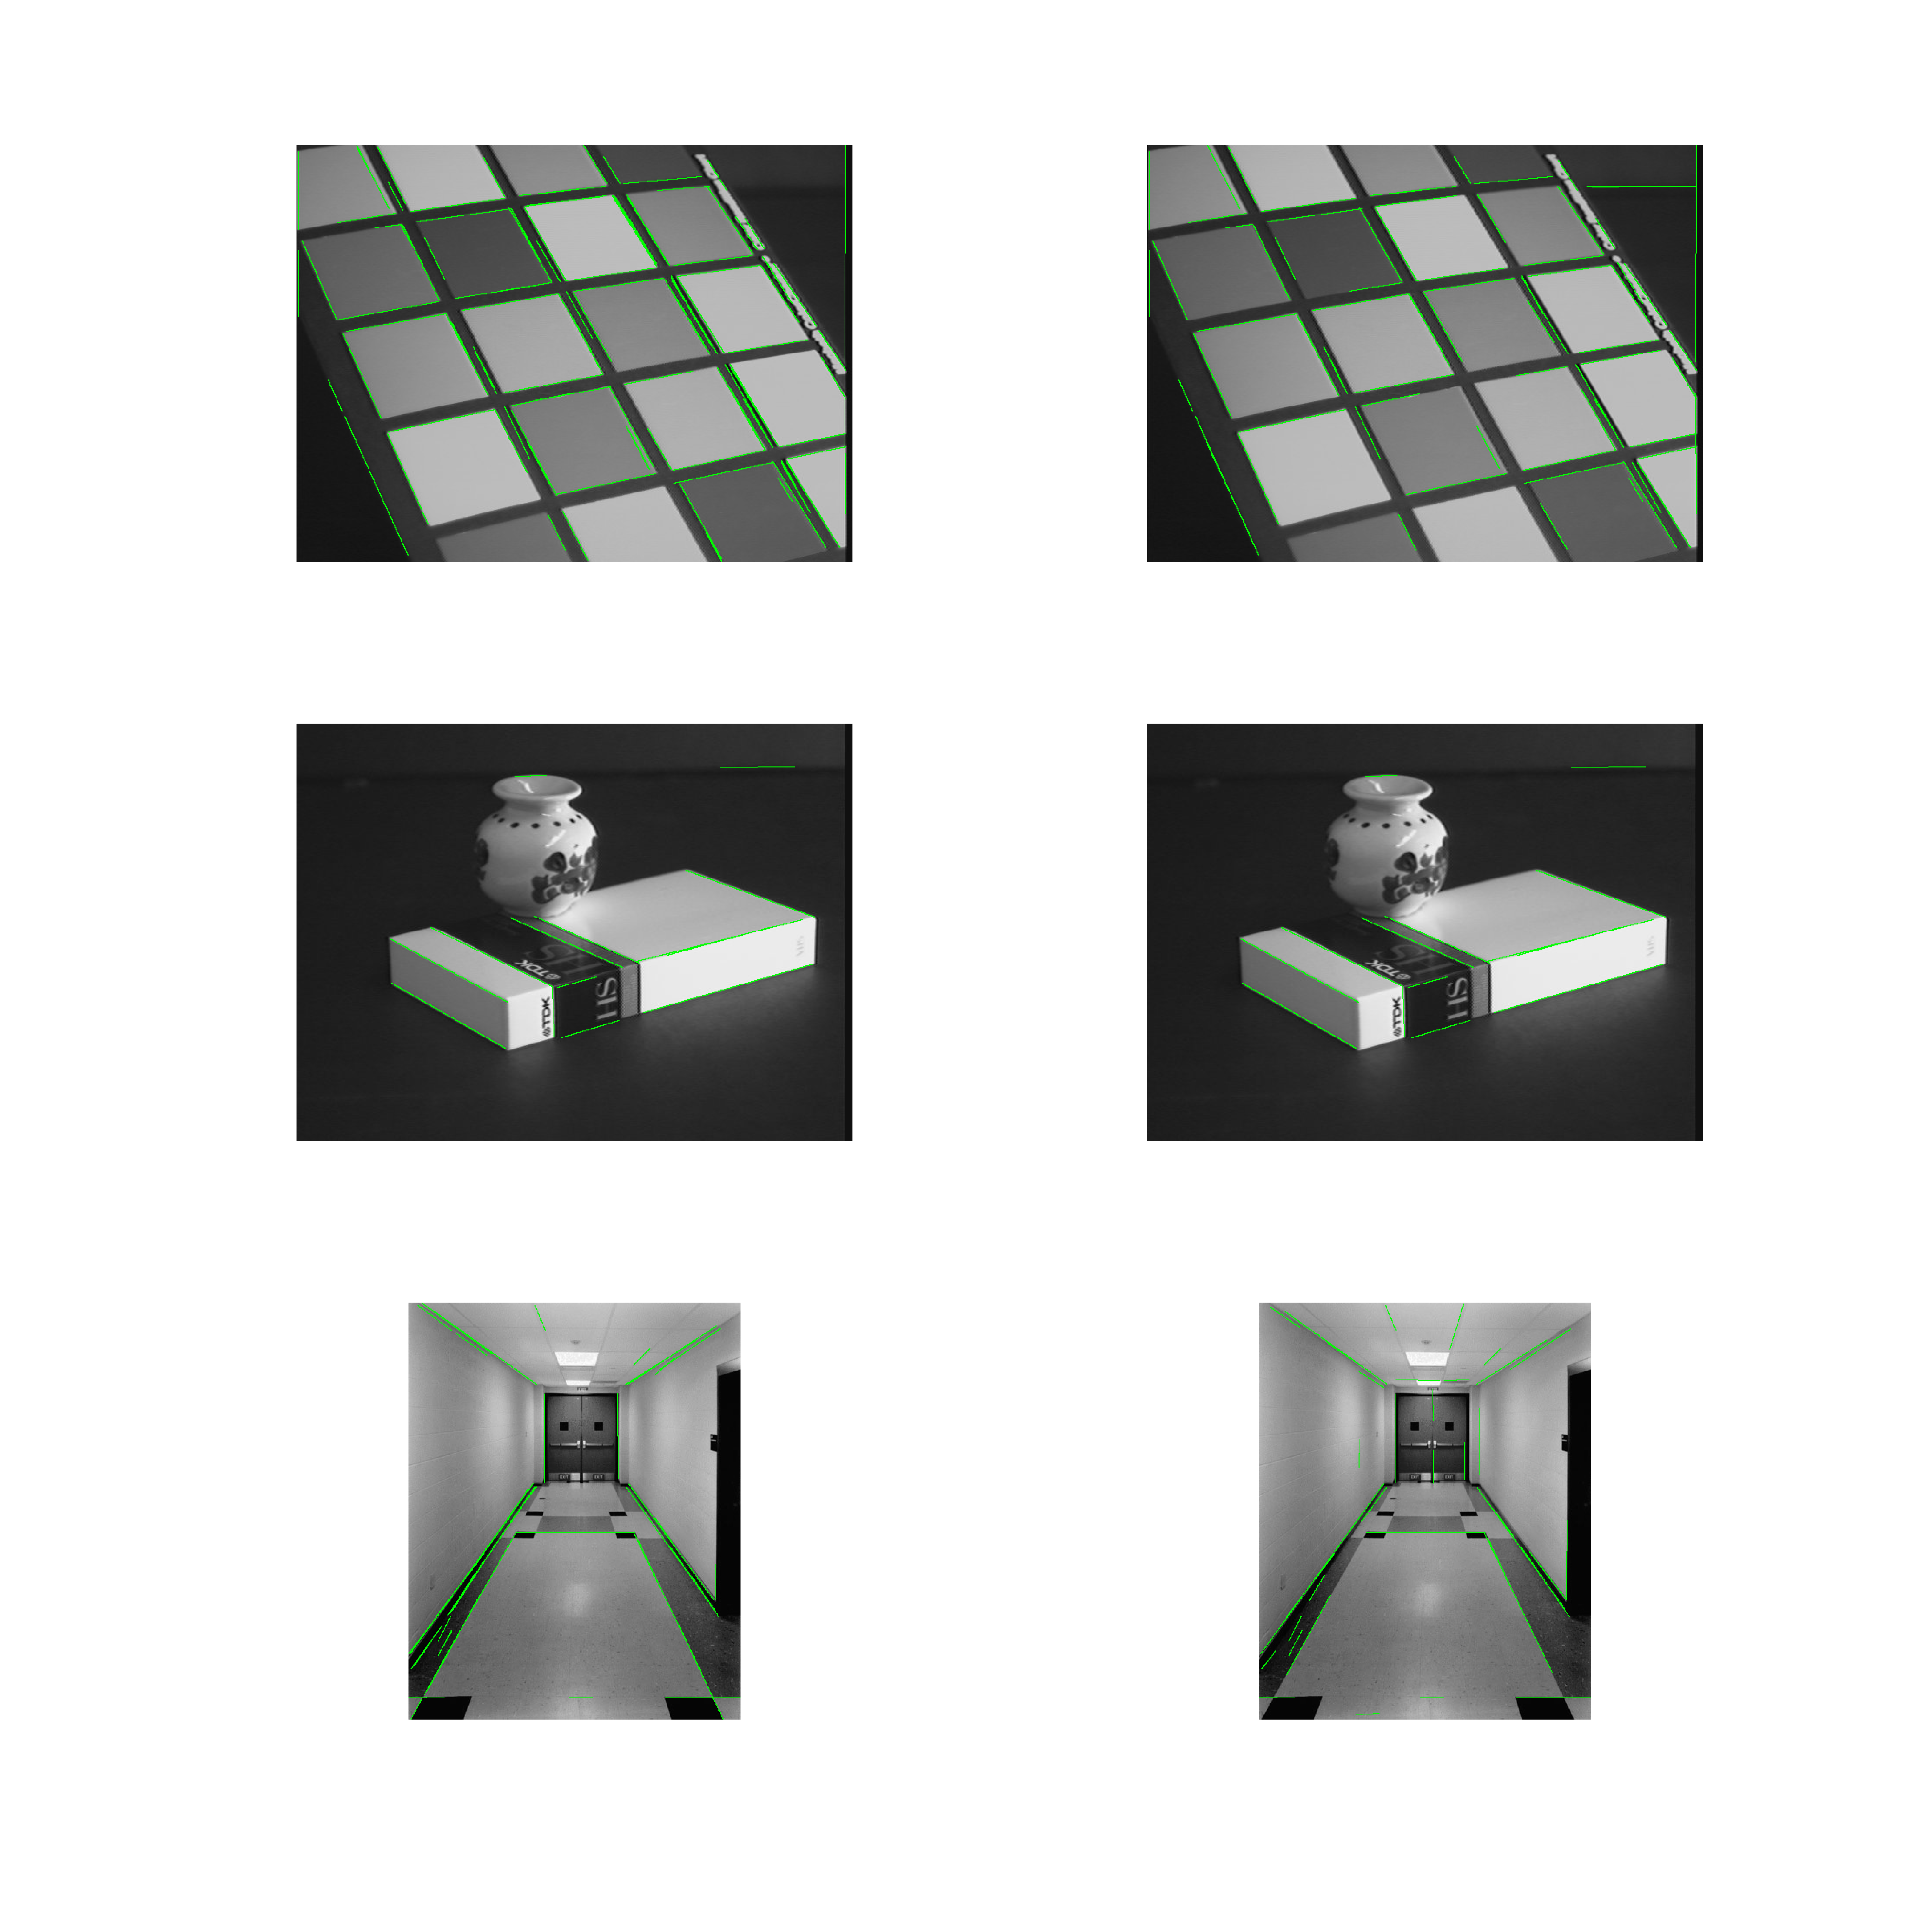
\includegraphics[width=0.85\linewidth]{hw4_3_1}
    \caption{results of extracting peaks from $H$ given images. 
    left: without applying NMS postprocessing; right: after applying NMS}
    \label{fig:5}
\end{figure}

As can be seen in Algorithm\ref{alg:2}, the default threshold for excluding the peaks below is set to $0.3 * max(H)$
and the default window size to be considered as "neighborhood" is set to $9 \times 9$. Thus changing these parameters
can affect the result of selected lines; if the threshold is too high or too low, it may exclude some lines or add 
unwanted minor lines. Growing the window size can be effective if the lines in the original image is scattered 
through entire image; if there exists lines that are close enough, with big window size, the lines can be skipped 
due to the suppression. On the other side, with smaller window size, the effect of NMS can be diminished; it might 
not remove the overlapped lines that are essentially the same. Adjusting the parameters on extracting the lines 
heavily depends on the images.

\figurename{\ref{fig:5}} shows the effect of applying NMS on peak extraction. It can be seen from
the left of \figurename{\ref{fig:5}} that the lines become thinner with some noisy lines suppressed.
Remaining results of the line detection from the images in data/ can be found in
results/*\_04lines.png. 

\section*{problem 4: hough circle transform}

The circle hough transform (CHT) is a specialization of hough transform, where the parametric equation
is based on circular equation. Given center point of a circle $(a, b)$ and $r$ as the radius, a circle
can be defined as:
\[(x-a)^2 + (y-b)^2 = r^2\]

By the circular equation above, $xy$-plane can be mapped to 3-dimensional $(a, b, r)$ space. 
As in \figurename{\ref{fig:6}}, possible circular candidates passing through the points in 
$xy$-plane can be mapped to the surface of an inverted cone having apex $(x, y, 0)$.

\begin{figure}[h]
    \centering
    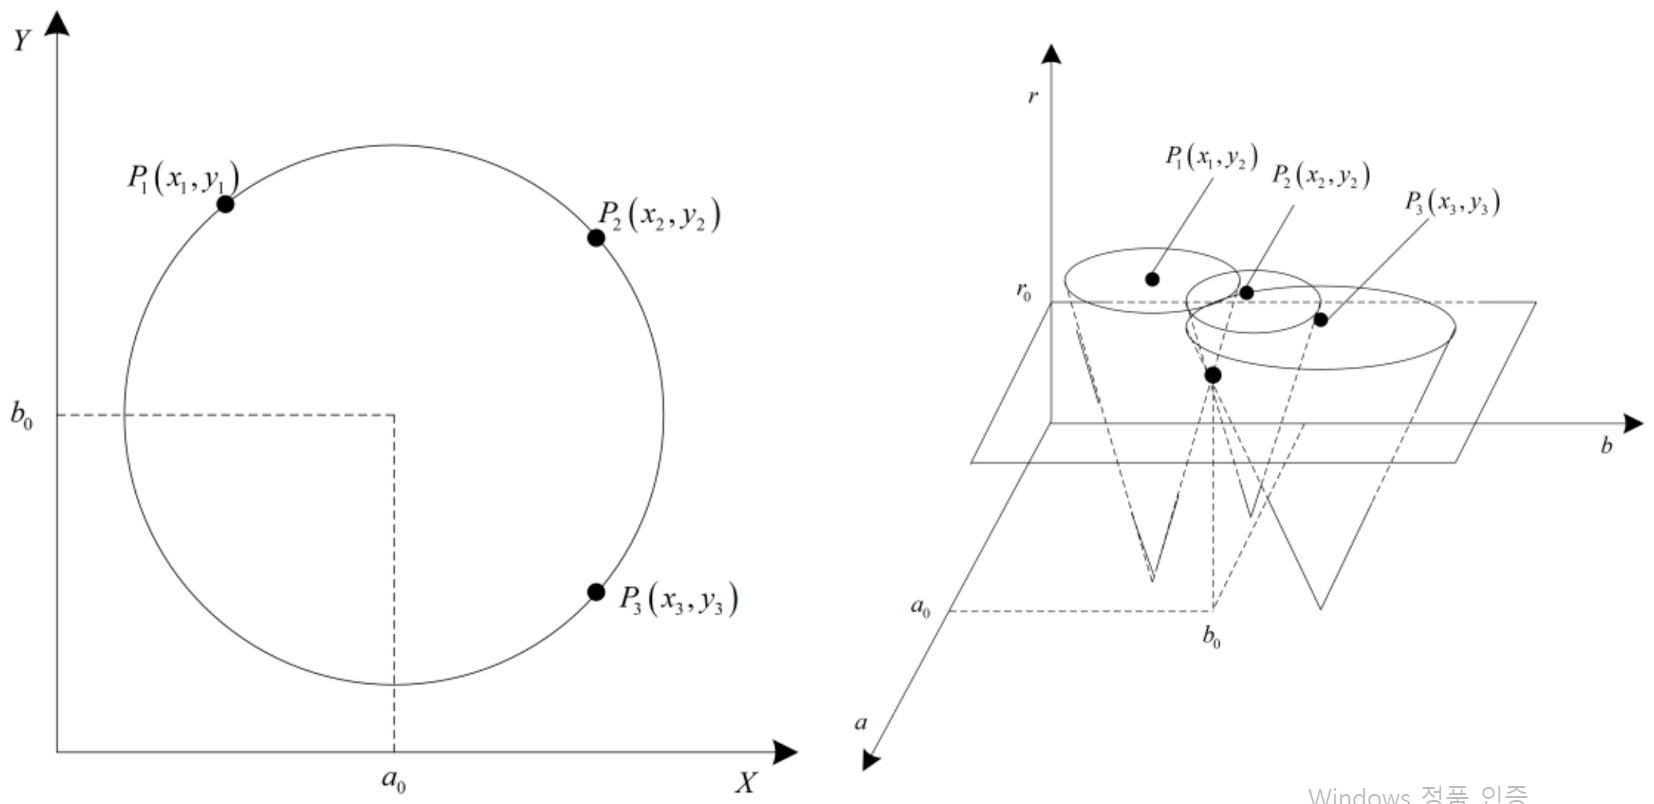
\includegraphics[width=\linewidth]{hw4_4_1}
    \caption{circular equation in $xy$ plane(left) and parametric space(right)}
    \label{fig:6}
\end{figure}

As in SHT, finding maximum intersections between the surfaces of the cones in $(a, b, r)$ space can be inverted
to the strong circular component in $xy$-plane. However, since the parametric space is 3-dimensional, there can be
several implementations for finding the parameter $(a, b, r)$. One of the implementation divides the process of
finding maximum intersections into two stages; first, with predefined radius, find the optimal center
of the circles from $ab$-plane, then find the optimal radius given the circle centers from $r$-line. 

\begin{figure}[h]
    \centering
    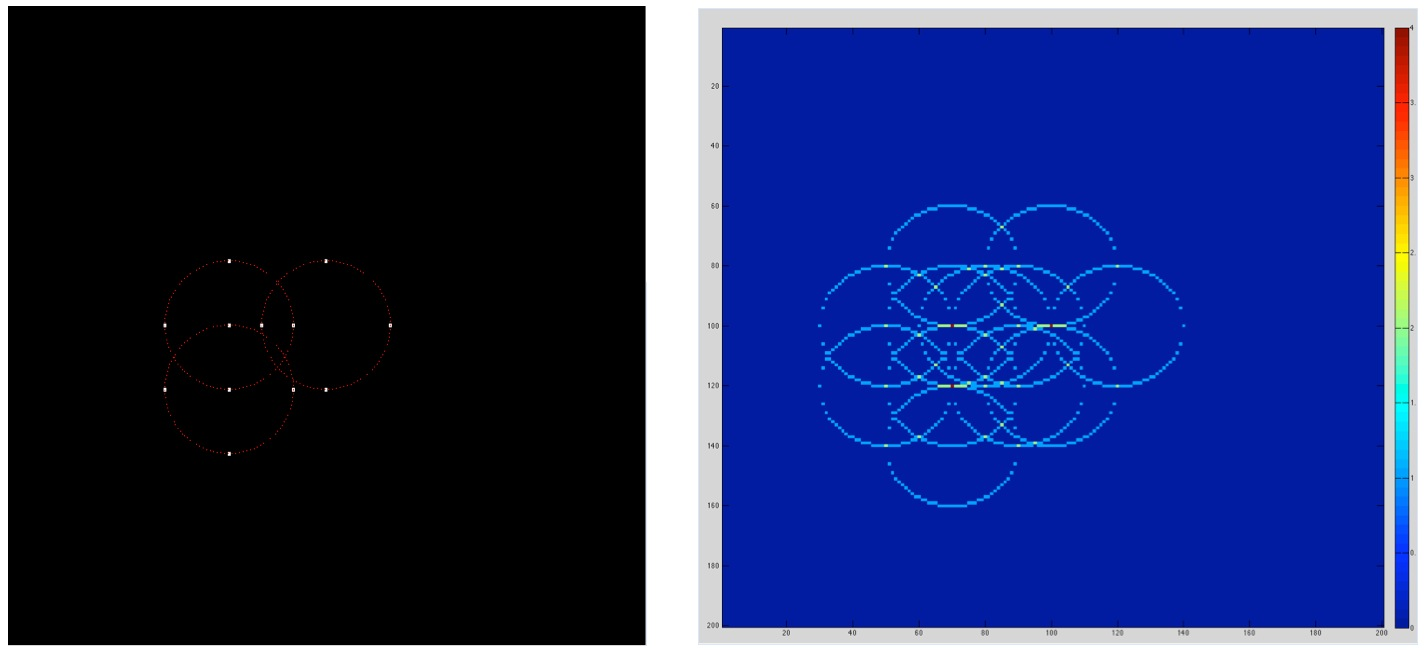
\includegraphics[width=\linewidth]{hw4_4_2}
    \caption{arbitrary points in $xy$-plane(left) and its parametric representation in $ab$-plane(right)
    assumed that the radius $r$ is known in advance}
    \label{fig:7}
\end{figure}

\figurename{\ref{fig:7}} shows the example of mapping between $xy$-plane and $ab$-plane with known radius $r$.
As in SHT, maximum intersection from the parametric representations, depicted as red dots in $ab$-plane,
can be inverted back to $xy$-plane defining the center of major circles from the scattered data.
Though this implementation need to have predefined radius to find the circle center and the accuracy of
detecting every circles in the image can depend on the hyperparameter, the process is done on either 2-dimensional
$ab$-plane or 1-dimensional $r$-line, making the implementation tractable with small memory footprint. 

In case the radius is unknown, iterating over 3-dimensional parametric space to find the maximum intersections
is also possible, while 3-dimensional accumulation is costly in terms of both memory and latency. 

\begin{figure}[h]
    \centering
    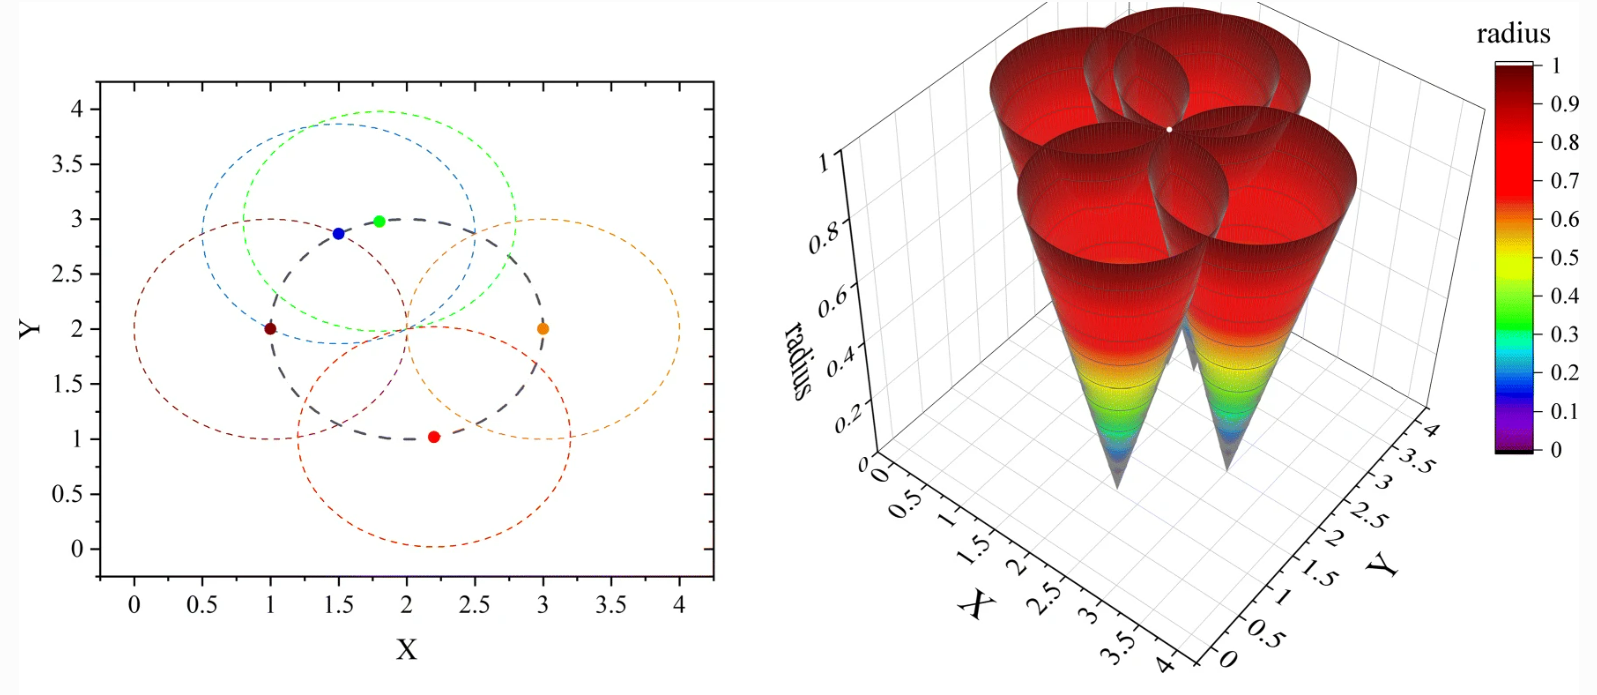
\includegraphics[width=\linewidth]{hw4_4_3}
    \caption{arbitrary points in $xy$-plane(left) and its parametric representation in $(a, b, r)$ space(right)}
    \label{fig:8}
\end{figure}

\figurename{\ref{fig:8}} shows the example of mapping between $xy$-plane and $(a, b, r)$ space. While dot in the
parametric space defines both the radius $r$ and the center of the circle $(a, b)$ in $xy$-plane.

\begin{figure}[h]
    \centering
    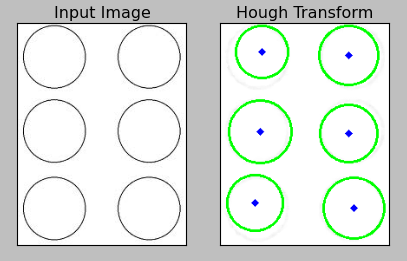
\includegraphics[width=\linewidth]{hw4_4_4}
    \caption{original image containing several circles and its CHT result}
    \label{fig:9}
\end{figure}

The example of applying CHT onto the image of multiple circles is shown in \figurename{\ref{fig:9}}. It can be 
seen that both circle center and its radius is approximated precisely.
Based on the parametric representation, ellipse, or any other form of structure would be able to be detected.

\end{document}
